\documentclass{article}

% if you need to pass options to natbib, use, e.g.:
% \PassOptionsToPackage{numbers, compress}{natbib}
% before loading nips_2018

% ready for submission
\usepackage{nips_2018}
\usepackage{enumitem}
% to compile a preprint version, e.g., for submission to arXiv, add
% add the [preprint] option:
%\usepackage[preprint]{nips_2018}

% to compile a camera-ready version, add the [final] option, e.g.:
% \usepackage[final]{nips_2018}

% to avoid loading the natbib package, add option nonatbib:
% \usepackage[nonatbib]{nips_2018}

\usepackage[utf8]{inputenc} % allow utf-8 input
\usepackage[T1]{fontenc}    % use 8-bit T1 fonts
\usepackage{hyperref}       % hyperlinks
\usepackage{url}            % simple URL typesetting
\usepackage{booktabs}       % professional-quality tables
\usepackage{amsfonts}       % blackboard math symbols
\usepackage{nicefrac}       % compact symbols for 1/2, etc.
\usepackage{microtype}      % microtypography
\usepackage{wrapfig}
\usepackage{picins}

\usepackage{amsmath}
\usepackage{amssymb}
\usepackage{amsthm}
\usepackage{algorithm}
\usepackage[noend]{algorithmic}
%\usepackage{algpseudocode}
\usepackage{graphicx}

\usepackage{natbib}

\usepackage[backgroundcolor = White,textwidth=2cm]{todonotes}
%\usepackage[disable,backgroundcolor = White,textwidth=\marginparwidth]{todonotes}
\newcommand{\todom}[2][]{\todo[color=orange!25,size=\small,#1]{G: #2}}
\newcommand{\todox}[2][]{\todo[color=purple!25,size=\small,#1]{K: #2}}
\newcommand{\todor}[2][]{\todo[color=blue!25,size=\small,#1]{R: #2}}
\setlength{\marginparwidth}{0.8in}


\renewcommand{\algorithmicrequire}{\textbf{Input:}}
\renewcommand{\algorithmicensure}{\textbf{Output:}}
\DeclareMathOperator*\argmin{arg\,min}
\DeclareMathOperator*\argmax{arg\,max}
\DeclareMathOperator*\sgn{sgn}
\DeclareMathOperator*\pr{Pr}
\DeclareMathOperator*\ep{\mathbb{E}}
\DeclareMathOperator\oep{\mathbb{E}}

\newcommand*{\refPi}{\bar{\pi}}
\newcommand*{\optPiRef}{\bar{\pi}_{\tau}^*}
\newcommand*{\cP}{\mathcal{P}}
\newcommand*{\cH}{\mathcal{H}}
\newcommand{\KL}{D_{\text{KL}}}
\newcommand{\ENT}{\text{ENT}}
\newcommand{\SR}{\text{SR}}
\newcommand{\pithetat}{\pi_{\theta_t}}

\newtheorem{thm}{Theorem}
\newtheorem{lem}{Lemma}
\newtheorem{defi}{Definition}
\newtheorem{prop}{Proposition}
\newtheorem{remk}{Remark}

\usepackage[capitalize]{cleveref}
\crefname{prop}{Proposition}{Propositions}
\crefname{thm}{Theorem}{Theorems}

%\title{Reversed Entropy Policy Mirror Descent for Reinforcement Learning}
\title{Policy Mirror Descent with Reversed KL Projection}

% The \author macro works with any number of authors. There are two
% commands used to separate the names and addresses of multiple
% authors: \And and \AND.
%
% Using \And between authors leaves it to LaTeX to determine where to
% break the lines. Using \AND forces a line break at that point. So,
% if LaTeX puts 3 of 4 authors names on the first line, and the last
% on the second line, try using \AND instead of \And before the third
% author name.

\author{
  David S.~Hippocampus\thanks{Use footnote for providing further
    information about author (webpage, alternative
    address)---\emph{not} for acknowledging funding agencies.} \\
  Department of Computer Science\\
  Cranberry-Lemon University\\
  Pittsburgh, PA 15213 \\
  \texttt{hippo@cs.cranberry-lemon.edu} \\
  %% examples of more authors
  %% \And
  %% Coauthor \\
  %% Affiliation \\
  %% Address \\
  %% \texttt{email} \\
  %% \AND
  %% Coauthor \\
  %% Affiliation \\
  %% Address \\
  %% \texttt{email} \\
  %% \And
  %% Coauthor \\
  %% Affiliation \\
  %% Address \\
  %% \texttt{email} \\
  %% \And
  %% Coauthor \\
  %% Affiliation \\
  %% Address \\
  %% \texttt{email} \\
}

\begin{document}
% \nipsfinalcopy is no longer used

\maketitle

\begin{abstract}
Policy optimization is a basic problem in reinforcement learning. This paper provides Reversed Entropy Policy Mirror Descent (REPMD), achieving two properties that enhance on-line exploration: preventing early convergence to  sub-optimal policies, and monotonically increasing a performance measure. REPMD adopts maximum entropy exploration within the classic mirror descent framework, and updates policy by a reversed KL projection. This approach overcomes undesirable mode seeking behaviour, while still enjoying the policy improvement guarantee. Experiments on bandit and algorithmic tasks demonstrate that the proposed method achieves better exploration than both undirected maximum entropy exploration and directed exploration with standard entropy projection.% without justified monotonically increasing performance property.
\end{abstract}

\section{Introduction}
Model-free deep reinforcement learning (RL) has recently been demonstrated to successfully solve a wide range of difficult sequential decision making problems \cite{schulman2015trust,mnih2015human,silver2016mastering}. Policy based DRL approaches represent the learner's policy with a neural network, and directly optimizes the policy by gradient update with respect to the parameters of the neural network. While the great expressive power of neural networks helps in modelling complicated policies, it also significantly introduces additional complications in understanding the behavior of the model. 

In practice, policy based DRL is different than a traditional optimization problem, in the sense that the argument to be optimized, i.e. the policy, is also used to collect training data from the environment. This interaction may lead to lack of exploration, since the learner's policy may get stuck in a local optimum and fail to collect high reward trajectories, preventing any learning from useful signals.  An on-line learning algorithm should have the ability to explore the policy space properly and efficiently, to avoid getting trapped in a locally optima, while discovering the globally optimal policy quickly.

In this paper, we propose a method with a better exploration strategy, such that (a) it retains the exploration efficiency of existing methods; (b) it monotonically increases its chance of exploring trajectories generated by the optimal policies, or evolving closer to the optimal policies. Our proposed method Reversed Entropy Policy Mirror Descent (REPMD), takes both the entropy and relative entropy regularizers. Unlike common policy gradient based methods, REPMD is in a two-stage manner.  REPMD first updates the policy in the entire policy-simplex, ignoring the constraint induced by its parametrization, then a projection step is performed to update the policy in the parametrized policy space. Such a two-stage update guarantees REPMD to increase performance monotonically. The proposed REPMD method is then justified from both theoretical and empirical perspectives.

%Kullback–Leibler (KL) divergence

The rest of the paper is organized as follows. After introducing some basic knowledge of mirror descent, we propose the REPMD method in Section 2. We provide the analysis for the monotonically increasing performance property of REPMD in Section 3, and conduct experiments to validate our algorithm in Section 4. Some related work is discussed in Section 5, and the conclusion and directions for future work are presented in Section 6.

\subsection{Notations and Settings}

We consider finite horizon reinforcement learning settings with finite state and action spaces. The behavior of an agent is modelled by a policy $\pi(a|s)$, which estimates a probability distribution over a finite set of actions given an observed state. At each time step $t$, the agent takes an action $a_t$ by sampling from $\pi(a_t | s_t)$. The environment then returns a reward $r_t = r(s_t, a_t)$ and the next state $s_{t+1} = f(s_t, a_t)$, where $f$ is the transition function and it is not revealed to the agent. Given a trajectory, a sequence of states and actions $\rho=(s_1, a_1, \dots, a_{T-1}, s_T)$, the policy probability and the total reward of $\rho$ are defined as $\pi(\rho) = \prod_{t=1}^{T-1} \pi(a_t| s_t)$ and $r(\rho) = \sum_{t=1}^{T-1} r(s_t, a_t)$. We use $\Delta \triangleq \{ \pi | \sum_{\rho}{\pi(\rho)} = 1, \pi(\rho) \ge 0, \forall \rho \}$ to refer to the probabilistic simplex over all possible trajectories. For simplicity we also assume that the state transition function is deterministic, while our results can be easily extended to the general setting with random transition functions.

\section{Exploration in Policy Optimization}

Policy optimization has been widely used across reinforcement learning (RL) settings. Given a set of parametrized policy functions $\pi_\theta \in \Pi$, policy optimization aims to search the optimal policy $\pi_\theta^*$ that achieves the highest expected reward,
\begin{equation}
\label{max_expected_reward}
\begin{split}
	\pi_\theta^* \in \argmax_{\pi_\theta \in \Pi}{ \ep\limits_{\rho \sim \pi_\theta}{r(\rho)} } ,
\end{split}
\end{equation}
However, directly optimizing the expected reward can lead to a lack of exploration, and such learning algorithms usually converge to a sub-optimal policy.
Often, entropy regularization is proposed to mitigate the lack of exploration, leading to the following objective function,
\begin{equation}
\label{eq:max_expected_reward_plus_entropy}
\begin{split}
\max\limits_{\pi_\theta \in \Pi}{ \ep\limits_{\rho \sim \pi_\theta}{  r(\rho) } + \tau \mathcal{H}(\pi_\theta) } = 
\max\limits_{\pi_\theta \in \Pi}{ \ep\limits_{\rho \sim \pi_\theta}{ \left[ r(\rho) - \tau \log{\pi_\theta(\rho)} \right] } }.
\end{split}
\end{equation}
where $\tau$ is a non-negative temperature parameter to control the degree of exploration. Using sampled trajectories to solve the above maximum entropy exploration (MENT) problem \cref{eq:max_expected_reward_plus_entropy} is a classic policy gradient method, well known as REINFORCE \cite{williams1992simple,williams1991function}.

Although MENT assigns non-zero probability to every action, hence allowing it to be explored by $\pi_\theta$ in principle, such exploration is inherently \textit{undirected}, i.e., ``exploration is ensured only by randomness'' \cite{thrun1992efficient}. 
Recently, Nachum et al. \cite{nachum2017improving} proposed the under-appreciated reward exploration method (UREX) that provides extra guidance on the exploration probability, as follows:
\begin{equation}
\label{eq:urex_objective}
\begin{split}
\max\limits_{\pi_\theta \in \Pi}{ \ep\limits_{\rho \sim \pi_\theta}{  r(\rho)  - \tau \KL(\pi_\tau^* \| \pi_\theta) } },
\end{split}
\end{equation}
where $\pi_\tau^*(\rho) \triangleq \frac{\exp\left\{ r(\rho) / \tau \right\}}{ \sum_{\rho'}{ \exp\left\{ r(\rho') / \tau \right\} } }$ is the optimal policy of \cref{eq:max_expected_reward_plus_entropy} without the policy constraint $\Pi$. With $\KL(\pi_\tau^* \| \pi_\theta)$ as its regularizer, UREX tries to give larger probability values over high reward sampled trajectories to prevent $\pi_\theta$ from being too far away with $\pi_\tau^*$. Despite its efficiency in exploration, UREX suffers from two fundamental problems. On the one hand, it is not clear what the fixed point of UREX actually represents, as shown in \cref{prop:urex_fixedpoint}. On the other hand, there is no theoretical justification that UREX can monotonically increase the performance, which is favorable for any policy update methods. 
\begin{prop}
	\label{prop:urex_fixedpoint}
	The fixed point of UREX in \cref{eq:urex_objective} has the form
	\[
	\pi_\theta(\rho) = \frac{\tau \pi_\tau^*(\rho)}{\alpha - r(\rho)},
	\]
	where $\alpha$ is a constant such that $\sum_{\rho}{ \pi_\theta(\rho)} = 1$ and $ \max_{\rho}{ r(\rho) } + \tau \ge \alpha \ge  \max\{\min_{\rho}{ r(\rho) } + \tau, \max_{\rho}{ r(\rho) } \}$.
\end{prop}
\begin{proof}
See the appendix of \cite{nachum2017improving}.
\end{proof}

\section{Reversed Entropy Policy Mirror Descent}
In this section we firstly discuss relative entropy regularization for policy based reinforcement learning and its relationship with mirror descent, paving the path for presenting our proposed Reversed Entropy Policy Mirror Descent (REPMD) algorithm. 

\subsection{Policy Mirror Descent}
\label{sec:pmd}
We first present a basic policy optimization algorithm based on the idea of Mirror Descent (MD). MD has been widely used in the literature of online learning and constrained optimization problems \cite{nemirovskii1983problem,beck2003mirror}. In particular, given a \emph{reference policy} $\refPi$, let 
\[
\ENT(\pi_\theta; \tau, \refPi) = { \ep\limits_{\rho \sim \pi_\theta}{  r(\rho)  - \tau \KL(\pi_\theta \| \refPi) } }.
\]
The MD update for policy optimization problem is 
\begin{equation}
\label{eq:max_expected_reward_plus_relative_entropy}
\pi_{\theta_{t+1}} = \argmax\limits_{\pi_\theta \in \Pi}  \ENT(\pi_\theta; \tau, \pithetat), 
\end{equation}
which combines the expected reward \cref{max_expected_reward} with a relative entropy regularizer.
Similar ideas have also been explored in \cite{peters2007reinforcement,wierstra2008episodic,peters2010relative,schulman2015trust,montgomery2016guided,nachum2017trust,haarnoja2018soft,abdolmaleki2018maximum}. The following \cref{prop:mirrordescent_projection} suggests an efficient implementation of the mirror descent algorithm.

\begin{prop}
	\label{prop:mirrordescent_projection}
	Given a \emph{reference policy} $\refPi$, define $\bar{\pi}_\tau^*(\rho) =  \frac{\refPi(\rho) \exp\left\{ r(\rho) / \tau \right\}}{ \sum_{\rho^{\prime}}{\refPi(\rho^{\prime}) \exp\left\{ r(\rho^{\prime}) / \tau \right\} } }$, then
	\[
	\argmax\limits_{\pi_\theta \in \Pi}{\ENT(\pi_\theta; \tau, \refPi)}= \argmin\limits_{\pi_\theta \in \Pi}{ \KL(\pi_\theta \| \bar{\pi}_\tau^*) } ,
	\]
\end{prop}
%\vspace{-0.2in}
\begin{proof}
	$-\tau \KL(\pi_\theta \| \bar{\pi}_\tau^*) = - \tau \sum_{\rho}{ \pi_\theta(\rho) \log \pi_\theta(\rho) } + \tau \sum_{\rho}{ \pi_\theta(\rho) (\log \refPi(\rho) + r(\rho) / \tau ) }  - Z_{\refPi} = \ep_{\rho \sim \pi_\theta}{  r(\rho)  - \tau \KL(\pi_\theta \| \refPi) } - Z_{\refPi}$. Note the fact that $Z_{\refPi} \triangleq \tau \log{ \sum_{\rho}{\refPi(\rho) \exp\left\{ r(\rho) / \tau \right\} } }$ is indenpendent of $\pi_\theta$ given the reference policy $\refPi$.
\end{proof}
Based on \cref{prop:mirrordescent_projection}, policy mirror descent (PMD) updates the policy $\pi_{\theta_{t+1}}$ by
\begin{equation}
\label{eq:pmd}
\begin{split}
&\argmin\limits_{\pi_\theta \in \Pi}{\KL( \pi_\theta \| \bar{\pi}_{\tau}^* )}, \\
\text{where}\ \ \bar{\pi}_{\tau}^* & =  \argmax\limits_{\pi \in \Delta}{ \ep\limits_{\rho \sim \pi}{  r(\rho)  - \tau \KL(\pi \| \pi_{\theta_t}) } }.
\end{split}
\end{equation}
One can show that Mirror descent asymptotically converges to the optimal policy when $\Pi$ is a convex set \cite{nemirovskii1983problem,beck2003mirror}. However, in practice, the policy $\pi_\theta$ is often parameterized by a complex non-linear function, such as a neural network, which does not satisfy the convex constraint set assumption. The next proposition shows that despite of the non-convexity of $\Pi$, the MD update can still improve the expected reward monotonically.
\begin{prop}
	\label{prop:monoto_policymirrordescent}
	Assume that $\pi_{\theta_{t}}$ is the update sequence of the policy mirror descent algorithm, then 
\[
\oep_{\rho \sim \pi_{\theta_{t+1}}}{r(\rho)} - \oep_{\rho \sim \pi_{\theta_{t}}}{  r(\rho)} \ge 0.
\] 
\end{prop}
\begin{proof}
	Note that $\KL(\pi_{\theta_{t+1}} \| \bar{\pi}_\tau^*)  = \min_{\pi_\theta \in \Pi}{ \KL(\pi_\theta \| \bar{\pi}_\tau^*)} \leq \KL(\pi_{\theta_{t}} \| \bar{\pi}_\tau^*)$. By expanding the KL divergence and rearranging terms, we have $ \tau \KL(\pi_{\theta_{t+1}} \| \pi_{\theta_{t}}) - \sum_{\rho}{ \pi_{\theta_{t+1}}(\rho) r(\rho) } \leq - \sum_{\rho}{ \pi_{\theta_{t}}(\rho) r(\rho) }$, which gives $\ep_{\rho \sim \pi_{\theta_{t+1}}}{  r(\rho)} - \ep_{\rho \sim \pi_{\theta_{t}}}{  r(\rho)} \geq \tau \KL(\pi_{\theta_{t+1}} \| \pi_{\theta_{t}}) \geq 0$.
\end{proof}

Although PMD enjoys this beneficial property, it is also well known that minimizing the KL divergence $\KL(\pi_\theta \| \bar{\pi}_\tau^*) $ is \emph{mode seeking} \cite{kevin2012machine}, which can cause mode collapse during the learning process. Once the policy $\bar{\pi}_\tau^*$ drops some of the modes, learning could be trapped into sub-optimal policies. Moreover, PMD is also prone to converging to local optima:
Note that the learning in \cref{eq:pmd} may converge to the policy $\pithetat$ that is a local maximizer of $\ep_{\rho \sim \pi} r(\rho)$. 
Since $\KL(\pi \| \pithetat) = 0$ for such policy, the learning algorithm has no incentive for further exploration, and thus will become trapped at a local optimum.
To overcome these drawbacks, we propose two modifications for the PMD algorithm, leading to our new algorithm.

\subsection{Reversed Entropy Policy Mirror Descent}
\label{sec:repmd}
The new algorithm, called Reversed Entropy Policy Mirror Descent (REPMD), instead solves the following optimization problem to update the policy $\pi_{\theta_{t+1}}$:
\begin{equation}
\label{eq:repmd}
\begin{split}
&\argmin\limits_{\pi_\theta \in \Pi}{\KL(\bar{\pi}_{\tau,\tau^{\prime}}^* \| \pi_\theta) }, \\
\text{where}\ \ \bar{\pi}_{\tau,\tau^{\prime}}^* & =  \argmax\limits_{\pi \in \Delta}{ \ep\limits_{\rho \sim \pi}{  r(\rho)  - \tau \KL(\pi \| \pi_{\theta_t}) + \tau^{\prime} \cH(\pi)} }.
\end{split}
\end{equation}
First, an additional entropy regularizer, controlled by a separate parameter $\tau^{\prime}\geq 0$, is added to the objective, which encourages additional exploration as in MENT. 
Second, we employ the reversed \emph{mean seeking} direction of KL divergence $\KL(\bar{\pi}_{\tau,\tau^{\prime}}^* \| \pi_\theta)$ to update the policy. 
The idea of optimizing this direction of KL divergence has proven to be effective for structured prediction and reinforcement learning in previous work, such as reward augmented maximum likelihood \cite{norouzi2016reward} and UREX \cite{nachum2017improving}.

A similar monotonic improvement result to \cref{prop:monoto_policymirrordescent} can also be proved for REPMD but only on the $\SR(\pi_\theta) $, as shown in \cref{thm:monotonically_increasing_sr_property}, where we let
\[
\SR(\pi_\theta) \triangleq (\tau + \tau^{\prime})\log{ \sum_{\rho}{ \exp\left\{ \frac{r(\rho) + \tau \log{\pi_\theta(\rho)} }{\tau + \tau^{\prime}} \right\} }}
\]
denote the softmax approximated expected reward of $\pi_\theta$.
%\todor[]{Why it is a sum over $\rho$ rather than expectation?}
\begin{thm}
	\label{thm:monotonically_increasing_sr_property}
	Assume that $\pi_{\theta_{t}}$ is the update sequence of the reversed entropy policy mirror descent algorithm, then 
	\[
	\SR(\pi_{\theta_{t+1}}) - \SR(\pithetat)\ge 0.
	\] 
\end{thm}
\begin{proof}
	Using $\KL(\pi_{\tau,\tau^{\prime}}^* \| \pi_{\theta_{t+1}}) = \min_{\pi_\theta \in \Pi}{ \KL(\pi_{\tau,\tau^{\prime}}^* \| \pi_\theta)} \le \KL(\pi_{\tau,\tau^{\prime}}^* \| \pithetat)$ and Jensen's inequality,
	\begin{equation*}
	\begin{split}
	&\SR(\pi_{\theta_{t+1}}) - \SR(\pithetat) = (\tau + \tau^{\prime}) \log{ \sum\limits_{\rho}{ \frac{  \exp\left\{ \frac{r(\rho) + \tau \log{\pi_{\theta_{t+1}}(\rho)} }{\tau + \tau^{\prime}} \right\}  }{ \sum\limits_{\rho}{  \exp\left\{ \frac{r(\rho) + \tau \log{\pithetat(\rho)} }{\tau + \tau^{\prime}} \right\} } }  } } \\
	=& (\tau + \tau^{\prime}) \log{ \sum\limits_{\rho}{ \frac{  \exp\left\{ \frac{r(\rho) + \tau \log{\pithetat(\rho)} }{\tau + \tau^{\prime}} \right\}  }{ \sum\limits_{\rho}{  \exp\left\{ \frac{r(\rho) + \tau \log{\pithetat(\rho)} }{\tau + \tau^{\prime}} \right\} } }  } \cdot \exp\left\{ \frac{\tau \log{\pi_{\theta_{t+1}}(\rho)} - \tau \log{\pithetat(\rho)} }{\tau + \tau^{\prime}} \right\} } \\
	=& (\tau + \tau^{\prime}) \log{ \sum\limits_{\rho}{ \pi_{\tau,\tau^{\prime}}^*(\rho) } \cdot \exp\left\{ \frac{\tau \log{\pi_{\theta_{t+1}}(\rho)} - \tau \log{\pithetat(\rho)} }{\tau + \tau^{\prime}} \right\} } \\
	\ge& (\tau + \tau^{\prime}) \sum\limits_{\rho}{ \pi_{\tau,\tau^{\prime}}^*(\rho) \log{ \exp\left\{ \frac{\tau \log{\pi_{\theta_{t+1}}(\rho)} - \tau \log{\pithetat(\rho)} }{\tau + \tau^{\prime}} \right\} } } \\
	=& \tau \sum\limits_{\rho}{ \pi_{\tau,\tau^{\prime}}^*(\rho) \log{ \frac{\pi_{\theta_{t+1}}(\rho)}{\pithetat(\rho)} } } = \tau \left[ \KL(\pi_{\tau,\tau^{\prime}}^* \| \pithetat) - \KL(\pi_{\tau,\tau^{\prime}}^* \| \pi_{\theta_{t+1}})\right] \ge 0. \qedhere
	\end{split}
	\end{equation*}
\end{proof}

Theorem \ref{thm:monotonically_increasing_sr_property} implies that the fixed points of REPMD have a correspondence with the stationary point of $\text{SR}(\pi_\theta)$. 
Although $\text{SR}(\pi_\theta)$ is different than the expected reward $\ep_{\rho \sim \pi_\theta}{r(\rho)}$,  we argue that $\SR(\pi_\theta)$ is still a reasonable performance measure. In fact, by properly adjusting the two temperature parameters $\tau$ and $\tau^{\prime}$, $\SR(\pi_\theta)$ recovers several existing performance measures, as shown in \cref{prop:sr}.
\begin{prop}
	\label{prop:sr}
	$\SR(\pi_\theta)$ satisfies the following properties:
	\begin{enumerate}[label=(\roman*)]
		\item  $\SR(\pi_\theta) \to \max_{\rho}{r(\rho)}$, as $\tau \to 0, \tau^{\prime} \to 0$.
		\item $\SR(\pi_\theta) \to \ep_{\rho \sim \pi_\theta}{r(\rho)}$, as $\tau \to \infty, \tau^{\prime} \to 0$. 
	\end{enumerate}	
\end{prop}
\begin{proof}
	To prove (i), note that as $\tau \to 0$, $\SR(\pi_\theta) \to \tau^{\prime} \log{ \sum_{\rho}{ \exp\left\{ \frac{r(\rho) }{ \tau^{\prime} } \right\} }}$, the standard softmax value. Taking limit on $\tau'$ gives the hardmax value $\max_{\rho}{r(\rho)}$ as $\tau^{\prime} \to 0$.
	
	To prove (ii), we have 
\begin{align*}
&\lim\limits_{\tau \to \infty}{ (\tau + \tau^{\prime})\log{ \sum_{\rho}{ \exp\{ \frac{r(\rho) + \tau \log{\pi_\theta(\rho)} }{\tau + \tau^{\prime}} \} }} } = {\scalebox{.95} {$\lim\limits_{\tau \to \infty}{ \frac{ \sum_{\rho}{ \pi_\theta(\rho) \exp\{ \frac{r(\rho) - \tau^{\prime} \log{\pi_\theta(\rho)} }{\tau + \tau^{\prime}} \} \left( r(\rho) - \tau^{\prime}\log{\pi_\theta(\rho)} \right) } }{  \sum_{\rho}{ \pi_\theta(\rho) \exp\{ \frac{r(\rho) - \tau^{\prime} \log{\pi_\theta(\rho)} }{\tau + \tau^{\prime}} \} } } }$ } }\\
&= \sum_{\rho}{ \pi_\theta(\rho) \left( r(\rho) - \tau^{\prime}\log{\pi_\theta(\rho)} \right) } = \ep_{\rho \sim \pi_\theta}{r(\rho)} + \tau^{\prime} \mathcal{H}(\pi_\theta)
 \end{align*}
 	As $\tau^{\prime} \to 0$, $\SR(\pi_\theta) \to \ep_{\rho \sim \pi_\theta}{r(\rho)}$.
\end{proof}

\begin{wrapfigure}{r}{0.5\textwidth}
    \begin{minipage}{0.5\textwidth}
      \begin{algorithm}[H]
  \caption{\label{alg:repmd}  The REPMD algorithm}
 \begin{algorithmic}[1]
  \INPUT $\tau, \tau', K$
  \OUTPUT  Policy $\pi_\theta$
  \STATE Random initialized $\pi_{\theta_1}$;
  \FOR { $t=1,2,\ldots, T$ }
  \STATE Set $\refPi = \pithetat$;
  \REPEAT 
  \STATE Sample a mini-batch of $K$ trajectories from $\refPi$;
  \STATE Compute the gradient according to \cref{eq:gradient_estimator};
  \STATE Update $\pi_{\theta_{t+1}}$ by the gradient;
  \UNTIL converged or reach max\_iter;
  \ENDFOR
  \STATE Return $\pi_{\theta_T}$.
 \end{algorithmic}
\end{algorithm}
    \end{minipage}
  \end{wrapfigure}
  
Note that $\text{SR}(\pi_\theta)$ also resembles ``softmax value function'' that appeared in value based RL \cite{nachum2017bridging,haarnoja2018soft,NIPS2017_6874}. The standard soft value can be recovered by $\text{SR}(\pi_\theta)$ as a special case when $\tau = 0$ or $\tau'=0$. 

According to \cref{prop:sr}, one should gradually decrease $\tau^{\prime}$ to reduce the level of exploration as sufficient reward landscape information has been collected during the learning process. Now we can make different choices for $\tau$, depending on the policy constraint set $\Pi$.

\begin{remk}
	\label{small_tau_choices}
	Using very small $\tau$ value, i.e., $\tau \to 0$, given $\tau^{\prime} \to 0$ and the reward landscape has been sufficiently explored, the constructed unconstrained policy $\bar{\pi}_{\tau,\tau^{\prime}}^* \to \pi^*$, where $\pi^*$ is the global deterministic optimal policy. Solving the projection $\pi_\theta \leftarrow \argmin_{\pi_\theta \in \Pi}{\KL(\bar{\pi}_{\tau,\tau^{\prime}}^* \| \pi_\theta}) \approx \argmin_{\pi_\theta \in \Pi}{\KL(\pi^* \| \pi_\theta})$, we actually obtain $\pi_\theta$ policy by directly projecting $\pi^*$ into $\Pi$. When the policy constraint $\Pi$ has additional nice properties, such as convexity, that support good behavior of KL projection, this should be a good choice.
\end{remk}
  
However, in practice, $\Pi$ is typically nonconvex, even when $\pi_\theta$ is parameterized by a linear function approximator, let alone more complex function approximations like a neural network. In such cases, the small $\tau$ value suggested in Remark \ref{small_tau_choices} might not work very well, since directly projecting $\pi^*$ into $\Pi$ might not always lead to a $\pi_\theta$ with large expected reward.

\begin{remk}
	\label{large_tau_choices}
	Given $\tau^{\prime} \to 0$ and a sufficiently explored reward landscape, as $\tau \to \infty$, the stationary point set of $\SR(\pi_\theta)$ will approach the stationary point set of $\sum_{\rho}{ \pi_\theta(\rho) r(\rho) }$.
\end{remk}

Remark \ref{large_tau_choices} indicates that during learning, $\pi_\theta$ may get stuck around some local maximum of $\SR(\pi_\theta)$, and increasing the $\tau$ value will lead to a different contour of $\SR(\pi_\theta)$, which might help $\pi_\theta$ escape to alternative local maxima. There exists an ideal sequence of $\tau$ values and $\tau \to \infty$ that make $\pi_\theta$ finally converge to $\pi_\theta^* \in \argmax_{\pi_\theta}{ \sum_{\rho}{\pi_\theta(\rho) r(\rho)} }$, i.e., the optimal policy in $\Pi$ with highest expected reward, recovering the target of policy optimization \cref{max_expected_reward}. A principled way to find such an ideal sequence of $\tau$ is under investigation.

\subsection{Learning}

We discuss some implementation details of REPMD. The full algorithm is presented in \cref{alg:repmd}.
First note that the \emph{unconstrained optimal policy} $\bar{\pi}_{\tau,\tau^{\prime}}^*$ in (\ref{eq:repmd}) has a closed form expression.
\begin{lem}
	\label{lem:opt_pi_ref}
	The unconstrained optimal policy of \cref{eq:repmd} has the following closed form expression:
	\[
	\bar{\pi}_{\tau,\tau^{\prime}}^*(\rho) \triangleq \frac{\refPi(\rho) \exp\left\{ \frac{r(\rho)-\tau^{\prime} \log \refPi(\rho) }{ \tau+\tau^{\prime}} \right\}}{ \sum_{\rho^{\prime}}{\refPi(\rho^{\prime}) \exp\left\{ \frac{r(\rho^{\prime})-\tau^{\prime} \log \refPi(\rho^{\prime})}{ \tau+\tau^{\prime}} \right\} } }.
	\] 
\end{lem}
\begin{proof}
	Rewrite the objective function defined in \cref{eq:repmd},
	\begin{equation}
	\ep\limits_{\rho \sim \pi} r(\rho)  - \tau \KL(\pi \| \refPi) + \tau^{\prime} \cH(\pi) = \ep\limits_{\rho \sim \pi} [r(\rho) + \tau \log \refPi(\rho)] + (\tau+\tau^{\prime}) \cH(\pi),
	\end{equation}
	which is an entropy regularized reshaped reward objective. The optimal policy of this objective can be obtained by directly applying Lemma 4 of \cite{nachum2017bridging}, i.e.
	\begin{equation}
	\bar{\pi}_{\tau,\tau^{\prime}}^*(\rho)\propto \exp\left\{ \frac{r(\rho)+\tau \log \refPi(\rho)}{\tau+\tau^{\prime}} \right\} = \refPi(\rho) \exp\left\{ \frac{r(\rho)-\tau^{\prime} \log \refPi(\rho)}{\tau+\tau^{\prime}} \right\}. \qedhere
	\end{equation}
\end{proof}
The REPMD objective in \cref{eq:repmd} can be easily optimized via stochastic gradient descent, given one can sample trajectories from $\bar{\pi}_{\tau,\tau^{\prime}}^*$.
Following the idea of UREX \cite{nachum2017improving}, we approximate the KL divergence using self-normalized importance sampling \citep{owen2013monte},
\begin{equation}
\label{eq:importance_sampling_kl}
\KL(\bar{\pi}_{\tau,\tau^{\prime}}^* \| \pi_\theta) = \ep_{\rho \sim \bar{\pi}_{\tau,\tau^{\prime}}^* } \left[ \log \bar{\pi}_{\tau,\tau^{\prime}}^*(\rho) - \log \pi_\theta(\rho) \right] = \ep_{\rho\sim \refPi} \frac{\bar{\pi}_{\tau,\tau^{\prime}}^*(\rho)}{\refPi(\rho)} \left[ \log \bar{\pi}_{\tau,\tau^{\prime}}^*(\rho) - \log \pi_\theta(\rho) \right].
\end{equation}

We can draw $K$ \textit{i.i.d.} samples $\{\rho_1, \dots, \rho_K\}$ from the \emph{reference policy} $\refPi$, and then approximate the gradient of $\KL(\bar{\pi}_{\tau,\tau^{\prime}}^* \| \pi_\theta)$ by averaging these $K$ samples according to \cref{eq:importance_sampling_kl}. 

\begin{thm}
	\label{thm:repmdgradientestimate}
	Let $\omega_k = \frac{r(\rho_k) - \tau^{\prime} \log{\refPi(\rho_k)} }{\tau + \tau^{\prime}}
$. Given $K$ \emph{i.i.d.} samples $\{\rho_1, \dots, \rho_K\}$ from the \emph{reference policy} $\refPi$, we have the following unbiased gradient estimator,
	\begin{equation}
	\label{eq:gradient_estimator}
	\nabla_{\theta} \text{\em KL}(\bar{\pi}_{\tau,\tau^{\prime}}^* \| \pi_\theta)\approx -\sum\limits_{k=1}^K{ \frac{ \exp\left\{ \omega_k \right\} }{ \sum_{j=1}^K{ \exp\left\{ \omega_j \right\}}} \nabla_{\theta} \log{\pi_\theta(\rho_k)} },
	\end{equation}
%	where 
%	\[
%	\omega_k = \frac{r(\rho_k) - \tau^{\prime} \log{\refPi(\rho_k)} }{\tau + \tau^{\prime}}.
%	\] 
\end{thm}
\begin{proof}
	According to \cref{eq:importance_sampling_kl} we have,
	\begin{equation}
	\begin{split}
	&\nabla_{\theta} \KL(\bar{\pi}_{\tau,\tau^{\prime}}^* \| \pi_\theta) \approx -\frac{1}{K}\sum_{k=1}^K \frac{\bar{\pi}_{\tau,\tau^{\prime}}^* (\rho_k)}{\refPi(\rho_k)} \nabla_{\theta} \log \pi_\theta(\rho_k) \\ 
	\approx & -\frac{1}{K}\sum_{k=1}^K \frac{\exp \{\omega_k\}} {\frac{1}{K} \sum_{j=1}^K \exp \{\omega_j\}} \nabla_{\theta} \log \pi_\theta(\rho_k) =  -\sum\limits_{k=1}^K{ \frac{ \exp\left\{ \omega_k \right\} }{ \sum_{j=1}^K{ \exp\left\{ \omega_j \right\}}} \nabla_{\theta} \log{\pi_\theta(\rho_k)} } \qedhere.
	\end{split}
	\end{equation}
\end{proof}

%

\if0
%Generally, the expected reward is estimated using mean sampled reward,
%\begin{equation}
%\label{mean_sampled_reward}
%\begin{split}
%	\ep\limits_{\rho \sim \pi_\theta}{r(\rho)} \approx \frac{1}{K} \sum\limits_{k=1}^{K}{ r(\rho_k)},
%\end{split}
%\end{equation}

In practice, solving (\ref{max_expected_reward}) is different with solving an optimization problem, in the sense that the argument to be optimized, $\pi_\theta$, is also used to sample trajectories. This issue may lead to lack of exploration. Intuitively, during the process of solving (\ref{max_expected_reward}), $\pi_\theta$ may be too close to the boundary of probabilistic simplex, i.e., the probabilities of choosing some actions are too small, and unfortunately, those actions may be followed by trajectories with high reward. In this case, $\pi_\theta$ has little chance to collect those high reward trajectories, and thus cannot learn from them.

To mitigate lack of exploration, entropy regularizer is combined with the expected reward objective to make $\pi_\theta$ have non-zero probability value for each action,
\begin{equation}
\label{max_expected_reward_plus_entropy}
\begin{split}
	\max\limits_{\pi_\theta \in \Pi}{ \ep\limits_{\rho \sim \pi_\theta}{  r(\rho) } + \tau \mathcal{H}(\pi_\theta) } = 
	\max\limits_{\pi_\theta \in \Pi}{ \ep\limits_{\rho \sim \pi_\theta}{ \left[ r(\rho) - \tau \log{\pi_\theta(\rho)} \right] } }.
\end{split}
\end{equation}

where $\tau$ is a non-negative temperature parameter to control the degree of exploration. Using sampled trajectories to solve the above MENT (maximum entropy exploration) problem (\ref{max_expected_reward_plus_entropy}) is the classic policy gradient method, well known as REINFORCE \cite{williams1992simple,williams1991function}.

Although MENT makes every action have non-zero probability to be explored by $\pi_\theta$, its exploration is actually \textit{undirected}, i.e., ``exploration is ensured only by randomness'' \cite{thrun1992efficient}. To see this, consider $\pi_\theta$ initialized as the uniform policy, with sample probability for each trajectory. Since the number of optimal trajectories is very small comparing with the total trajectory number, it is very likely that $\pi_\theta$ collects some suboptimal trajectories with moderate or low rewards. After some gradient updates, $\pi_\theta$ will have higher probability values for those trajectories with moderate rewards. And for the next sampling round, it is more likely that $\pi_\theta$ will collect some suboptimal trajectories. Repeatedly sampling and updating in this way, the policy gradient method may lead $\pi_\theta$ quickly converge to some local optimal policies with undesirable expected reward. At this point, since $\pi_\theta$ has low probability values for optimal trajectories, the only chance for exploration is fortunate or randomness.

The main disadvantage of undirected exploration is that the current policy $\pi_\theta$ has no knowledge of the optimal policy $\pi_\theta^*$. A good exploration strategy should endow the policy ability of exploring optimal trajectories, i.e., those trajectories generated by the optimal policies. Recently, Nachum et al. \cite{nachum2017improving} proposed the UREX (under-appreciated reward exploration) method,
\begin{equation}
\label{urex_objective}
\begin{split}
	\max\limits_{\pi_\theta \in \Pi}{ \ep\limits_{\rho \sim \pi_\theta}{  r(\rho)  - \tau \KL(\pi_\tau^* \| \pi_\theta) } },
\end{split}
\end{equation}
where $\pi_\tau^*(\rho) \triangleq \frac{\exp\left\{ \frac{r(\rho)}{\tau} \right\}}{ \sum\limits_{\rho}{ \exp\left\{ \frac{r(\rho)}{\tau} \right\} } }$ is the optimal policy of (\ref{max_expected_reward_plus_entropy}) without the policy constraint $\Pi$.

With $\KL(\pi_\tau^* \| \pi_\theta)$ as its regularizer, UREX tries to give larger probability values over high reward sampled trajectories as well as prevent $\pi_\theta$ from being too far away with $\pi_\tau^*$. However, UREX has its own disadvantages. \textit{On the one hand}, the fixed point of UREX update, $\pi_\theta(\rho) = \frac{\tau \pi_\tau^*(\rho)}{\alpha - r(\rho)}$, cannot be determined even $\tau$ is given, i.e., $\alpha$ should be chosen to satisfy $\sum_{\rho}{ \pi_\theta(\rho)} = 1$ and $\alpha > \max_{\rho}{ r(\rho) }$. The first condition cannot provide any information with respect to the optimal choice of $\alpha$, which makes choosing $\alpha$ heuristic. While the second condition need knowledge of maximum trajectory reward, which in practice is usually impossible. \textit{On the other hand}, there is no theoretical justification that UREX has the monotonically increasing performance property, which is favorable for any policy update methods. Suppose the current policy can evolve to a policy with better performance somehow, then its chance for exploring the optimal trajectories will increase, since the new policy is closer to the optimal policies under certain performance measures.

As aforementioned, reasonable exploration strategies should have the abilities of (a) exploring enough actions, or avoiding approaching the boundary of the probabilistic simplex too early; (b) increasing its chance of exploring trajectories generated by the optimal policies, or evolving closer to the optimal policies in some sense. In this paper, we propose our PMD (projected mirror descent) method, achieving (a) by using entropy regularizer as in MENT; (b) by employing similar update strategy as MD (mirror descent) in the probabilistic simplex. PMD takes both the KL (Kullback–Leibler) divergence in MD and the entropy regularizer in MENT as its regularizer mixture. Unlike policy gradient based methods, PMD updates the policy by projection, which is necessary to guarantee the monotonically increasing performance property. The proposed PMD method is then justified from both the theoretical and the empirical perspectives.

The rest of the paper is organized as follows. After introducing some basic knowledge of mirror descent, we propose our PMD method in Section 2. We provide the analysis for the monotonically increasing performance property of PMD in Section 3, and conduct experiments to validate our algorithm in Section 4. Some related work is discussed in Section 5, and the conclusion and future work are presented in Section 6.

\subsection{Notations and Settings}

We consider reinforcement learning settings with finite horizon, finite state and action space. The behavior of an agent is modeled by a policy $\pi(a|s)$, which outputs probability distribution over all the action $a$ given any observed state $s$. At each time step $t$, the agent takes an action $a_t$ by sampling from $\pi(a_t | s_t)$. The environment then returns a reward $r_t = r(s_t, a_t)$ and the next state $s_{t+1} = f(s_t, a_t)$, where $f$ is the transition function and it is not revealed to the agent. Given a trajectory, which is a sequence of states and actions $\rho=(s_1, a_1, \dots, a_{T-1}, s_T)$, the policy probability of $\rho$ is defined as $\pi(\rho) = \prod_{t=1}^{T-1} \pi(a_t| s_t)$, and the total reward of $\rho$ is $r(\rho) = \sum_{t=1}^{T-1} r(s_t, a_t)$. $\Delta \triangleq \{ \pi | \sum_{\rho}{\pi(\rho)} = 1, \pi(\rho) \ge 0, \forall \rho \}$ refers to the probabilistic simplex over all possible trajectories. 

Let $h$ denote the latent variable of the environment which decides both the initial state $s_1$ and the state transition function of the environment. 
For simplicity we also assume that the state transition function is deterministic. 
Our results can be easily extended to the general setting with random transition functions.

\section{Projected Mirror Descent}
In this section, we firstly discuss relative entropy regularization for policy based reinforcement learning and its relationship with mirror descent, paving the path for presenting our proposed Projected Mirror Descent (PMD) algorithm. Consider the following objective function which combines the expected reward (\ref{max_expected_reward}) with a relative entropy regularizer given fixed \emph{reference policy} $\refPi$,
\begin{equation}
\label{max_expected_reward_plus_relative_entropy}
\begin{split}
	\max\limits_{\pi_\theta \in \Pi}{ \ep\limits_{\rho \sim \pi_\theta}{  r(\rho)  - \tau \KL(\pi_\theta \| \refPi) } }
\end{split}
\end{equation}
The above objective implies an iterative algorithm to learn the policy $\pi_\theta$, i.e., at each iteration $t$, one can fix the current policy $\pithetat$ as the \emph{reference policy}, and calculate $\pi_{\theta_{t+1}}$ by solving (\ref{max_expected_reward_plus_relative_entropy}). In fact, this update strategy refers to the MD (mirror descent) algorithm in online convex optimization \cite{}. Note that the objective in (\ref{max_expected_reward_plus_relative_entropy}) can be rewritten as the KL divergence,
\begin{prop}
Define $\bar{\pi}_\tau^*(\rho) \triangleq \frac{\refPi(\rho) \exp\left\{ \frac{r(\rho)}{\tau} \right\}}{ \sum_{\rho^{\prime}}{\refPi(\rho^{\prime}) \exp\left\{ \frac{r(\rho^{\prime})}{\tau} \right\} } }$. (\ref{max_expected_reward_plus_relative_entropy}) is equivalent with
$\min\limits_{\pi_\theta \in \Pi}{ \tau \KL(\pi_\theta \| \bar{\pi}_\tau^*) } $.
\label{prob1}
\end{prop}
%\vspace{-0.2in}
\begin{proof}
$-\tau \KL(\pi_\theta \| \bar{\pi}_\tau^*) = - \tau \sum_{\rho}{ \pi_\theta(\rho) \log \pi_\theta(\rho) } + \tau \sum_{\rho}{ \pi_\theta(\rho) (\log \refPi(\rho) + r(\rho) / \tau ) }  - Z_{\refPi} = \ep_{\rho \sim \pi_\theta}{  r(\rho)  - \tau \KL(\pi_\theta \| \refPi) } - Z_{\refPi}$. Note the fact that $Z_{\refPi} \triangleq \tau \log{ \sum_{\rho}{\refPi(\rho) \exp\left\{ r(\rho) / \tau \right\} } }$ is indenpendent of $\pi_\theta$ given the reference policy $\refPi$.
\end{proof}

The objective $\KL(\pi_\theta \| \bar{\pi}_\tau^*)$ indicates another implementation of mirror descent, i.e., at each iteration $t$, one can fix the current policy $\pithetat$ as the reference policy $\refPi$, and then construct an \emph{unconstrained optimal policy} $\bar{\pi}_\tau^*$, and calculate $\pi_{\theta_{t+1}} \leftarrow \argmin_{\pi_\theta \in \Pi}{ \KL(\pi_\theta \| \bar{\pi}_\tau^*) }$. 


Given the policy constraint $\Pi$ is a convex set, mirror descent can guarantee asymptotically convergence to the optimal policy \cite{}. While in practice, the policy $\pi_\theta$ is often parameterized by a complex non-linear function, such as neural networks. Therefore, the convexity of $\Pi$ is no longer satisfied. However, one can still show the MD update can improve the expected reward monotonically.

\begin{prop}
Mirror descent can increase the expected reward monotonically. 
\end{prop}
\begin{proof}
Using $\KL(\pi_{\theta_{t+1}} \| \bar{\pi}_\tau^*)  = \min_{\pi_\theta \in \Pi}{ \KL(\pi_\theta \| \bar{\pi}_\tau^*)} \leq \KL(\pi_{\theta_{t}} \| \bar{\pi}_\tau^*)$, expanding the KL divergence and rearranging terms, $ \tau \KL(\pi_{\theta_{t+1}} \| \pi_{\theta_{t}}) - \sum_{\rho}{ \pi_{\theta_{t+1}}(\rho) r(\rho) } \leq - \sum_{\rho}{ \pi_{\theta_{t}}(\rho) r(\rho) }$, which gives $\ep_{\rho \sim \pi_{\theta_{t+1}}}{  r(\rho)} - \ep_{\rho \sim \pi_{\theta_{t}}}{  r(\rho)} \geq \tau \KL(\pi_{\theta_{t+1}} \| \pi_{\theta_{t}}) \geq 0$.
\end{proof}

Although MD enjoys this nice property of monotonically increasing expected reward, it is well known that solving $\min_{\pi_\theta \in \Pi}{\KL(\pi_\theta \| \bar{\pi}_\tau^*)  } $ using stochastic gradient descent is challenging. The KL divergence $\KL(\pi_\theta \| \bar{\pi}_\tau^*) $ is known to be \emph{mode seeking} \cite{kevin2012machine}. Directly optimizing this direction of KL divergence could make the policy fall into local minima. Due to the effect of ignoring some modes of $\bar{\pi}_\tau^*$, sub-optimal policy would be pursued in each iteration of the optimization. To overcome the drawback of directly applying MD in policy based reinforcement learning, we propose the following PMD (projected mirror descent) method. The policy optimization problem of PMD is,
\begin{equation}
\label{pmd_obj}
\begin{split}
	&\min\limits_{\pi_\theta \in \Pi}{\KL(\bar{\pi}_{\tau,\tau^{\prime}}^* \| \pi_\theta) }, \\
	\text{where}\ \ \bar{\pi}_{\tau,\tau^{\prime}}^* &\triangleq \argmax\limits_{\pi \in \Delta}{ \ep\limits_{\rho \sim \pi}{  r(\rho)  - \tau \KL(\pi \| \refPi) + \tau^{\prime} \cH(\pi)} }.
\end{split}
\end{equation}

PMD differs with the original MD in two aspects. First, as in MENT, an entropy regularizer controlled by a separate parameter $\tau^{\prime}\geq 0$ is augmented to the objective in (\ref{max_expected_reward_plus_relative_entropy}) to encourage enough further exploration of the policy. In the case that $\tau^{\prime}=0$, i.e., there is no entropy regularization, the \emph{unconstrained optimal policy} $\bar{\pi}_{\tau,\tau^{\prime}}^*$ is identical as in MD. Second, we employ the reversed \emph{mean seeking} direction KL divergence $\KL(\bar{\pi}_{\tau,\tau^{\prime}}^* \| \pi_\theta)$ to update the policy, rather than the \emph{mode seeking} direction KL used in the original MD. The idea of optimizing this direction of KL divergence has proven to be effective for structured prediction and reinforcement learning in previous work, such as RAML (reward augmented maximum likelihood) \cite{norouzi2016reward} and UREX \cite{nachum2017improving}.

\subsection{Learning}
The \emph{unconstrained optimal policy} $\pi_{\tau,\tau^{\prime}}^*$ in (\ref{pmd_obj}) has closed form expression.
\begin{lem}
$\bar{\pi}_{\tau,\tau^{\prime}}^*(\rho) \triangleq \frac{\refPi(\rho) \exp\left\{ \frac{r(\rho)-\tau^{\prime} \log \refPi(\rho) }{ \tau+\tau^{\prime}} \right\}}{ \sum_{\rho^{\prime}}{\refPi(\rho^{\prime}) \exp\left\{ \frac{r(\rho^{\prime})-\tau^{\prime} \log \refPi(\rho^{\prime})}{ \tau+\tau^{\prime}} \right\} } }$ is the unconstrained optimal policy of (\ref{pmd_obj}).
\label{opt_pi_ref}
\end{lem}
\begin{proof}
First, rewrite the objective function defined in (\ref{pmd_obj}),
\begin{equation}
\ep\limits_{\rho \sim \pi} r(\rho)  - \tau \KL(\pi \| \refPi) + \tau^{\prime} \cH(\pi) = \ep\limits_{\rho \sim \pi} [r(\rho) + \tau \log \refPi(\rho)] + (\tau+\tau^{\prime}) \cH(\pi),
\end{equation}
which is an entropy regularized reshaped reward objective. The optimal policy of this objective can be obtained by directly applying Lemma 4 of \cite{nachum2017bridging}:
\begin{equation}
\bar{\pi}_{\tau,\tau^{\prime}}^*(\rho)\propto \exp\left\{ \frac{r(\rho)+\tau \log \refPi(\rho)}{\tau+\tau^{\prime}} \right\} = \refPi(\rho) \exp\left\{ \frac{r(\rho)-\tau^{\prime} \log \refPi(\rho)}{\tau+\tau^{\prime}} \right\}. \qedhere
\end{equation}
\end{proof}

It is straightforward to optimize the PMD objective (\ref{pmd_obj}) with stochastic gradient descent if one can sample from the policy $\bar{\pi}_{\tau,\tau^{\prime}}^*$. However, since the reward landscape is completely unknown in RL, directly sampling from $\bar{\pi}_{\tau,\tau^{\prime}}^*$ is intractable in practice. Following \cite{nachum2017improving}, we approximate the KL divergence using self-normalized importance sampling \cite{owen2013monte},
\begin{equation}
\label{importance_sampling_kl}
\KL(\bar{\pi}_{\tau,\tau^{\prime}}^* \| \pi_\theta) = \ep_{\rho \sim \bar{\pi}_{\tau,\tau^{\prime}}^* } \left[ \log \bar{\pi}_{\tau,\tau^{\prime}}^*(\rho) - \log \pi_\theta(\rho) \right] = \ep_{\rho\sim \refPi} \frac{\bar{\pi}_{\tau,\tau^{\prime}}^*(\rho)}{\refPi(\rho)} \left[ \log \bar{\pi}_{\tau,\tau^{\prime}}^*(\rho) - \log \pi_\theta(\rho) \right].
\end{equation}

We can draw $K$ \textit{i.i.d.} samples $\{\rho_1, \dots, \rho_K\}$ from the \emph{reference policy} $\refPi$, and then approximate the gradient of $\KL(\bar{\pi}_{\tau,\tau^{\prime}}^* \| \pi_\theta)$ by averaging these $K$ samples according to (\ref{importance_sampling_kl}). 

\begin{thm}
Define $\omega_k \triangleq \frac{r(\rho_k) - \tau^{\prime} \log{\refPi(\rho_k)} }{\tau + \tau^{\prime}}$. Given $K$ \emph{i.i.d.} samples $\{\rho_1, \dots, \rho_K\}$ from the \emph{reference policy} $\refPi$, we have the following unbiased gradient estimator,
\begin{equation}
\label{gradient_estimator}
\nabla_{\theta} \text{\em KL}(\bar{\pi}_{\tau,\tau^{\prime}}^* \| \pi_\theta)\approx -\sum\limits_{k=1}^K{ \frac{ \exp\left\{ \omega_k \right\} }{ \sum_{j=1}^K{ \exp\left\{ \omega_j \right\}}} \nabla_{\theta} \log{\pi_\theta(\rho_k)} }
\end{equation}
\end{thm}
\begin{proof}
According to (\ref{importance_sampling_kl}) we have,
\begin{equation}
\begin{split}
&\nabla_{\theta} \KL(\bar{\pi}_{\tau,\tau^{\prime}}^* \| \pi_\theta) \approx -\frac{1}{K}\sum_{k=1}^K \frac{\bar{\pi}_{\tau,\tau^{\prime}}^* (\rho_k)}{\refPi(\rho_k)} \nabla_{\theta} \log \pi_\theta(\rho_k) \\ 
%= & -\frac{1}{K}\sum_{k=1}^K \frac{\exp \{\omega_k\}} {\sum_{\rho} \refPi(\rho) \exp\{\omega_k\}} \nabla_{\theta} \log \pi_\theta(\rho_k)\\
\approx & -\frac{1}{K}\sum_{k=1}^K \frac{\exp \{\omega_k\}} {\frac{1}{K} \sum_{j=1}^K \exp \{\omega_k\}} \nabla_{\theta} \log \pi_\theta(\rho_k) =  -\sum\limits_{k=1}^K{ \frac{ \exp\left\{ \omega_k \right\} }{ \sum_{j=1}^K{ \exp\left\{ \omega_j \right\}}} \nabla_{\theta} \log{\pi_\theta(\rho_k)} } \qedhere
\end{split}
\end{equation}
\end{proof}

The proposed PMD algorithm can be outlined as follows: at each iteration $t$, PMD fixes the policy $\pithetat$ as the \emph{reference policy} $\refPi$ and construct the \emph{unconstrained optimal policy} $\bar{\pi}_{\tau, \tau^{\prime}}^*$. $\pi_{\theta_{t+1}}$ is obtained by solving $\min_{\pi_\theta \in \Pi}{\KL(\bar{\pi}_{\tau,\tau^{\prime}}^* \| \pi_\theta})$ using stochastic gradient descent, where the gradient is estimated by (\ref{gradient_estimator}) using $K$ \emph{i.i.d.}trajectories sampled from $\refPi$.

\section{Theoretical Analysis}

In PMD, we use the reversed $\KL(\pi_{\tau,\tau^{\prime}}^* \| \pi_\theta)$ as the objective, which is different with the original KL divergence in mirror descent. This modification will not make PMD have the same property of monotonically increasing expected reward. Alternatively, we prove that PMD increases the softmax approximated expected reward monotonically.
\begin{thm}
\label{monotonically_increasing_sr_property}
The projected mirror descent method can improve the softmax approximated expected reward $(\tau + \tau^{\prime})\log{ \sum\limits_{\rho}{ \exp\left\{ \frac{r(\rho) + \tau \log{\pi_\theta(\rho)} }{\tau + \tau^{\prime}} \right\} }}$ monotonically.
\end{thm}
\begin{proof}
Using $\KL(\pi_{\tau,\tau^{\prime}}^* \| \pi_{\theta_{t+1}}) = \min_{\pi_\theta \in \Pi}{ \KL(\pi_{\tau,\tau^{\prime}}^* \| \pi_\theta)} \le \KL(\pi_{\tau,\tau^{\prime}}^* \| \pithetat)$ and Jensen's inequality,
\begin{equation*}
\begin{split}
	&(\tau + \tau^{\prime}) \log{ \sum\limits_{\rho}{ \exp\left\{ \frac{r(\rho) + \tau \log{\pi_{\theta_{t+1}}(\rho)} }{\tau + \tau^{\prime}} \right\} }} - (\tau + \tau^{\prime}) \log{\sum\limits_{\rho}{  \exp\left\{ \frac{r(\rho) + \tau \log{\pithetat(\rho)} }{\tau + \tau^{\prime}} \right\} }} \\
	&= (\tau + \tau^{\prime}) \log{ \sum\limits_{\rho}{ \frac{  \exp\left\{ \frac{r(\rho) + \tau \log{\pi_{\theta_{t+1}}(\rho)} }{\tau + \tau^{\prime}} \right\}  }{ \sum\limits_{\rho}{  \exp\left\{ \frac{r(\rho) + \tau \log{\pithetat(\rho)} }{\tau + \tau^{\prime}} \right\} } }  } } \\
	&= (\tau + \tau^{\prime}) \log{ \sum\limits_{\rho}{ \frac{  \exp\left\{ \frac{r(\rho) + \tau \log{\pithetat(\rho)} }{\tau + \tau^{\prime}} \right\}  }{ \sum\limits_{\rho}{  \exp\left\{ \frac{r(\rho) + \tau \log{\pithetat(\rho)} }{\tau + \tau^{\prime}} \right\} } }  } \cdot \exp\left\{ \frac{\tau \log{\pi_{\theta_{t+1}}(\rho)} - \tau \log{\pithetat(\rho)} }{\tau + \tau^{\prime}} \right\} } \\
	&= (\tau + \tau^{\prime}) \log{ \sum\limits_{\rho}{ \pi_{\tau,\tau^{\prime}}^*(\rho) } \cdot \exp\left\{ \frac{\tau \log{\pi_{\theta_{t+1}}(\rho)} - \tau \log{\pithetat(\rho)} }{\tau + \tau^{\prime}} \right\} } \\
	&\ge (\tau + \tau^{\prime}) \sum\limits_{\rho}{ \pi_{\tau,\tau^{\prime}}^*(\rho) \log{ \exp\left\{ \frac{\tau \log{\pi_{\theta_{t+1}}(\rho)} - \tau \log{\pithetat(\rho)} }{\tau + \tau^{\prime}} \right\} } } \\
	&= \tau \sum\limits_{\rho}{ \pi_{\tau,\tau^{\prime}}^*(\rho) \log{ \frac{\pi_{\theta_{t+1}}(\rho)}{\pithetat(\rho)} } } = \tau \left[ \KL(\pi_{\tau,\tau^{\prime}}^* \| \pithetat) - \KL(\pi_{\tau,\tau^{\prime}}^* \| \pi_{\theta_{t+1}})\right] \ge 0. \qedhere
\end{split}
\end{equation*}
\end{proof}

Theorem \ref{monotonically_increasing_sr_property} implies that the fixed point set of the PMD update has a correspondence with the stationary point of $\SR(\pi_\theta) \triangleq (\tau + \tau^{\prime})\log{ \sum_{\rho}{ \exp\left\{ \frac{r(\rho) + \tau \log{\pi_\theta(\rho)} }{\tau + \tau^{\prime}} \right\} }}$, which we call it as the \textit{the softmax approximated expected reward}.

Although different with the expected reward $\ep_{\rho \sim \pi_\theta}{r(\rho)}$, the softmax approximated expected reward $\SR(\pi_\theta)$ is still a reasonable performance measure. By changing the two temperature parameters $\tau$ and $\tau^{\prime}$, this metric can recover several existing performance measures.

\begin{remk}
\label{sr_limits}
R1. $\text{\em SR}(\pi_\theta) \to \max_{\rho}{r(\rho)}$ as $\tau \to 0, \tau^{\prime} \to 0$.

R2. $\text{\em SR}(\pi_\theta) \to \ep_{\rho \sim \pi_\theta}{r(\rho)}$ as $\tau \to \infty, \tau^{\prime} \to 0$.
\end{remk}
\begin{proof}
R1. As $\tau \to 0$, $\SR(\pi_\theta) \to \tau^{\prime} \log{ \sum_{\rho}{ \exp\left\{ \frac{r(\rho) }{ \tau^{\prime} } \right\} }}$, the standard softmax value, the limit of which is the hardmax value $\max_{\rho}{r(\rho)}$ as $\tau^{\prime} \to 0$.

R2. $\lim\limits_{\tau \to \infty}{ (\tau + \tau^{\prime})\log{ \sum_{\rho}{ \exp\{ \frac{r(\rho) + \tau \log{\pi_\theta(\rho)} }{\tau + \tau^{\prime}} \} }} }
= \lim\limits_{\tau \to \infty}{ \frac{ \sum_{\rho}{ \pi_\theta(\rho) \exp\{ \frac{r(\rho) - \tau^{\prime} \log{\pi_\theta(\rho)} }{\tau + \tau^{\prime}} \} \left( r(\rho) - \tau^{\prime}\log{\pi_\theta(\rho)} \right) } }{  \sum_{\rho}{ \pi_\theta(\rho) \exp\{ \frac{r(\rho) - \tau^{\prime} \log{\pi_\theta(\rho)} }{\tau + \tau^{\prime}} \} } } }$
$= \sum_{\rho}{ \pi_\theta(\rho) \left( r(\rho) - \tau^{\prime}\log{\pi_\theta(\rho)} \right) } = \ep_{\rho \sim \pi_\theta}{r(\rho)} + \tau^{\prime} \mathcal{H}(\pi_\theta)$.

As $\tau^{\prime} \to 0$, $\SR(\pi_\theta) \to \ep_{\rho \sim \pi_\theta}{r(\rho)}$.
\end{proof}

According to Remark \ref{sr_limits}, we should gradually decrease $\tau^{\prime}$ to reduce the level of exploration as enough reward landscape information has been collected during the learning process. Now we can make different choices for $\tau$, depending on the policy constraint $\Pi$.

\begin{remk}
\label{small_tau_choices}
Using very small $\tau$ value, i.e., $\tau \to 0$, the constructed unconstrained policy $\pi_{\tau,\tau^{\prime}}^* \to \pi^*$, where $\pi^*$ is the global deterministic optimal policy, given $\tau^{\prime} \to 0$ and the reward landscape has been sufficiently explored. Solving the projection $\pi_\theta \leftarrow \argmin_{\pi_\theta \in \Pi}{\KL(\bar{\pi}_{\tau,\tau^{\prime}}^* \| \pi_\theta}) \approx \argmin_{\pi_\theta \in \Pi}{\KL(\pi^* \| \pi_\theta})$, we actually obtain $\pi_\theta$ policy by directly projecting $\pi^*$ into $\Pi$. When the policy constraint $\Pi$ has nice property, such as convexity, to support the good behavior of KL projection, this should be a good choice.
\end{remk}

However, in practice, $\Pi$ is often certain nonconvex, even if $\pi_\theta$ is parameterized by linear approximations, let alone more complex function approximations like neural networks. In this case, very small $\tau$ value choices suggested in Remark \ref{small_tau_choices} may not work very well, since directly projecting $\pi^*$ into $\Pi$ may not always lead to $\pi_\theta$ with high expected reward.
 
\begin{remk}
\label{large_tau_choices}
Given $\tau^{\prime} \to 0$ and the reward landscape has been sufficiently explored, as $\tau \to \infty$, the stationary point set of $\SR(\pi_\theta)$ will approach the stationary point set of $\sum_{\rho}{ \pi_\theta(\rho) r(\rho) }$.
\end{remk}

Remark \ref{large_tau_choices} indicates that during learning, $\pi_\theta$ may get stuck around some local maxima of $\SR(\pi_\theta)$, and increasing the $\tau$ value will lead to different contour of $\SR(\pi_\theta)$, which may help $\pi_\theta$ to get across the previous local maxima. There exists an ideal sequence of $\tau$ values and $\tau \to \infty$ to make $\pi_\theta$ finally converge to $\argmax_{\pi_\theta}{ \sum_{\rho}{\pi_\theta(\rho) r(\rho)} }$, i.e., the optimal policy in $\Pi$ with highest expected reward. A principled way to find such an ideal sequence of $\tau$ is under investigation.
\fi



%\begin{figure*}[t]
%\begin{minipage}{0.33\linewidth}
%\centering
%\includegraphics[width=1.8in]{./Bandit.png}
%%\caption{Error rate}
%%\label{a}
%%\centerline{(a) $M$=20}
%\end{minipage}%
%\begin{minipage}{0.33\linewidth}
%\centering
%\includegraphics[width=1.8in]{./Copy.png}
%%\caption{Error rate}
%%\label{a}
%%\centerline{(b) $M$=50}
%\end{minipage}%
%\begin{minipage}{0.33\linewidth}
%\centering
%\includegraphics[width=1.8in]{./DuplicatedInput.png}
%%\caption{Error rate}
%%\label{a}
%%\centerline{(c) $M$=100}
%\end{minipage}%
%
%\begin{minipage}{0.33\linewidth}
%\centering
%\includegraphics[width=1.8in]{./Copy.png}
%%\caption{Error rate}
%%\label{a}
%%\centerline{(a) $M$=20}
%\end{minipage}%
%\begin{minipage}{0.33\linewidth}
%\centering
%\includegraphics[width=1.8in]{./Copy.png}
%%\caption{Error rate}
%%\label{a}
%%\centerline{(b) $M$=50}
%\end{minipage}%
%\begin{minipage}{0.33\linewidth}
%\centering
%\includegraphics[width=1.8in]{./Copy.png}
%%\caption{Error rate}
%%\label{a}
%%\centerline{(c) $M$=100}
%\end{minipage}%
%
%\caption{We report the results with the best hyper-parameters for each method. Each plot shows average reward with standard error during training. Plot of synthetic bandit problem is averaged over 10 runs. Plots of algorithmic tasks are averaged across 25 random training runs (5 runs $\times$ 5 random seed for neural network initialization). The x-axis is number of sampled trajectories. } 
%\label{fig:results}
%\end{figure*}

\section{Experiments}
We present our experimental results in this section. REPMD is compared with standard policy based reinforcement learning algorithms on several different test domains.   
%We compare our proposed approach Reversed Entropy Policy Mirror Descent (REPMD) with standard policy based reinforcement learning algorithms on several different test domains.  

\subsection{Tasks}
We test the performance of REPMD on a synthetic bandit problem and the algorithmic tasks from OpenAI gym library \cite{1606.01540}.  
\subsubsection{Synthetic Bandit}

We develop a simple synthetic multi-armed bandit problem as an initial testbed. The problem has 10,000 distinct actions. The reward of each action $i$ is initialized by $r_i = s_i^{8}$, where $s_i$ is randomly sampled from a uniform distribution over $[0,1)$. We represent each action $i$ with a feature vector $\phi_i\in \mathbb{R}^{20}$, randomly sampled from a standard normal distribution. Let $\Phi=[\phi_1,\dots,\phi_{10,000}]$ denote the feature matrix. The policy is parameterized by a weight vector $\theta\in  \mathbb{R}^{20}$ and  defined by $\text{softmax}(\Phi^{\top}\theta)$. Note that we only learn the $\theta$ parameter, the features $\Phi$ are fixed during training. 

\subsubsection{Algorithmic Tasks}

We consider five algorithmic tasks, in rough order of difficulty: Copy, DuplicatedInput, RepeatCopy, Reverse, and ReversedAddition \cite{1606.01540}. In each problem, the agent operates on a tape of characters or digits. At each time step, the agent read one character or digit, and then decide to either move the read pointer one step in any direction of the tape, or write a character or digit to output. The total reward of each sampled trajectory is only observed at the end. The goal for each task is:
\begin{itemize}
\item \textbf{Copy:} Copy a sequence of characters to output. 
\item \textbf{DuplicatedInput:} Duplicate a sequence of characters.
\item \textbf{RepeatCopy:} Copy a sequence of characters, reverse it, then forward the sequence again. 
\item \textbf{Reverse:} Reverse a sequence of characters.
\item \textbf{ReversedAddition:} Observe two numbers in base 3 in little-endian order on a $2\times n$ grid tape. The agent should add the two numbers together. 
\end{itemize}
For all of these algorithmic tasks, the policy is parameterized by a recurrent neural network with LSTM cells of hidden dimension 128 \cite{hochreiter1997long}. 

%\subsection{Baselines}
%
%We implement Policy Mirror Descent (PMD) to prove the effectiveness of the \emph{mean seeking} direction of KL divergence for policy optimization used in REPMD. Like in REPMD, we augment a separate tempreture parameter $\tau'\geq 0$ to the original objective function (\ref{max_expected_reward_plus_relative_entropy}) of PMD, which gives $\max_{\pi_\theta \in \Pi}{ \ep_{\rho \sim \pi_\theta}{  r(\rho)  - \tau \text{KL}(\pi_\theta \| \refPi) } + \tau'\cH(\pi_\theta) }$, to encourage further exploration of the policy. 
%
%For synthetic bandit problem, we compare REPMD against PMD, REINFORCE with entropy regularization (MENT) \cite{williams1992simple,williams1991function}, and under-appreciated reward exploration (UREX)\cite{nachum2017improving}. For algorithmic tasks, we compare REPMD against PMD and UREX. We omit MENT since it has been shown less effective than UREX in algorithmic tasks \cite{nachum2017improving}. 

\begin{figure*}[t]
\begin{center}
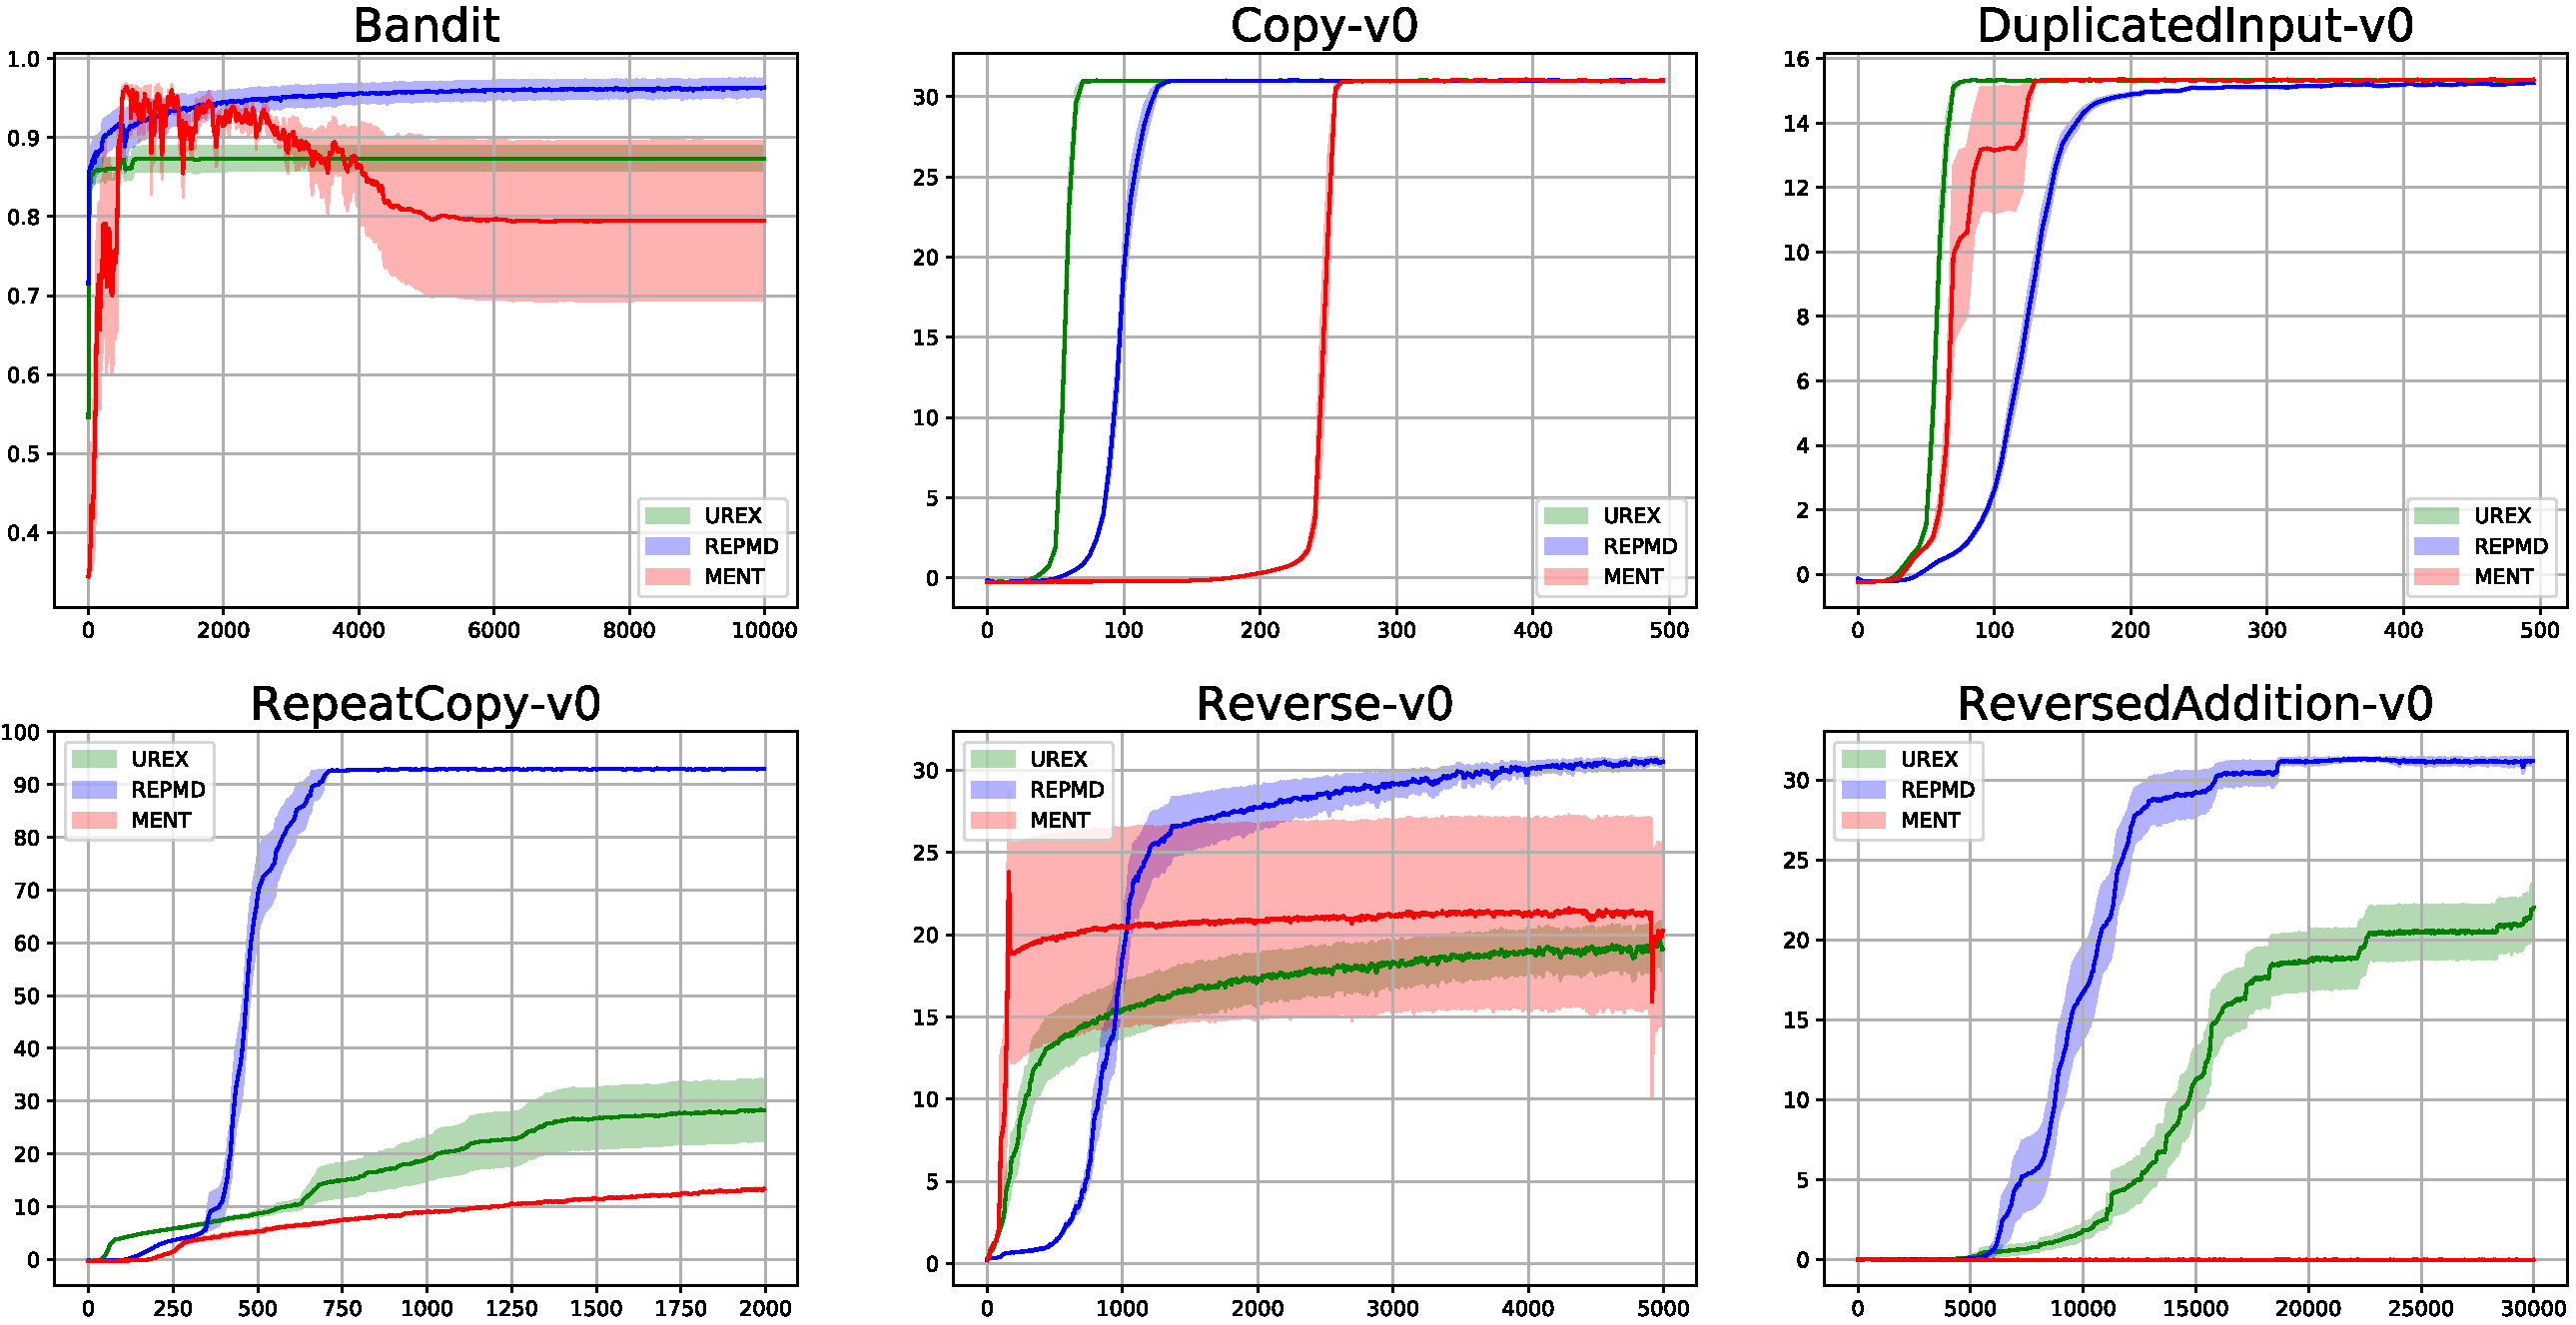
\includegraphics[width=0.85\linewidth]{./fig1.pdf}
\end{center}
\caption{
Results using the best hyper-parameters for each method: MENT (red), UREX (green), and REPMD (blue).
Plots show average reward with standard error during training. Synthetic bandit results averaged over 5 runs. Algorithmic task results averaged over 25 random training runs (5 runs $\times$ 5 random seeds for neural network initialization). X-axis is number of sampled trajectories. } 
\label{fig:results}
\end{figure*}

\subsection{Implementation Details}

As shown in \cref{alg:repmd}, the policy is updated by performing KL divergence projection using stochastic gradient descent (SGD). In our experiments, the end condition of SGD is controlled by two parameters: $\epsilon > 0$ and $\text{F\_STEP}\in \{0,1 \}$. First, SGD halts if the change of the KL divergence is below or equal to $\epsilon$. Second, $\text{F\_STEP}$ decides the maximum number of SGD steps. If $\text{F\_STEP}=1$, the maximum number is $\sqrt{t}$ at iteration $t$; while if $\text{F\_STEP}=0$, there is no restriction on the maximum number of gradient steps, and stopping condition of SGD only depends on $\epsilon$.

For the synthetic bandit problem, we explore the following main hyper-parameters: learning rate $\eta \in \{0.1, 0.01, 0.001\}$; entropy regularizer of UREX and MENT $\tau\in \{1.0, 0.5, 0.1, 0.05\}$; relative entropy regularizer of REPMD $\tau\in \{1.0, 0.5, 0.1, 0.05\}$; $\epsilon\in \{0.01, 0.005, 0.001\}$ and $\text{F\_STEP}\in \{0,1\}$ for the stop condition of SGD in REPMD. The entropy regularizer $\tau'$ of REPMD is set to 0.  

For the algorithmic tasks, $N$ distinct environments are used to generate samples. On each environment, $K$ random trajectories are sampled using the agent's policy to estimate gradient according to (\ref{eq:gradient_estimator}), which gives the batch size $N\times K$ in total. We apply the same batch training setting as in UREX \cite{nachum2017improving}, where $N=40$ and $K=10$. The following main hyper-parameters are explored: learning rate $\eta \in \{0.1, 0.01, 0.001\}$; relative entropy regularizer of REPMD $\tau\in \{1.0, 0.5, 0.1, 0.05\}$; entropy regularizer of REPMD $\tau'\in \{0, 0.01, 0.005, 0.001\}$; gradient clipped norm for training LSTM $c\in \{1, 10, 40, 100\}$; $\epsilon\in \{0.01, 0.005, 0.001\}$ and $\text{F\_STEP}\in \{0,1\}$ for the stopping condition of SGD in REPMD. Parameters of UREX are set according to the ones reported in \cite{nachum2017improving}. Implementations of all algorithm are based on the open source code by the author of UREX \footnote{\url{https://github.com/tensorflow/models/tree/master/research/pcl_rl}}.

\subsection{Comparative Evaluation}

For the synthetic bandit problem, we compare REPMD against REINFORCE with entropy regularization (MENT) \cite{williams1992simple} and under-appreciated reward exploration (UREX) \cite{nachum2017improving}. For the algorithmic tasks, we compare REPMD only against UREX, since UREX has been shown to  outperform MENT in these cases \cite{nachum2017improving}. The results are reported in Figure (\ref{fig:results}). It is clear that REPMD substantially outperforms the competitors on all of these benchmark tasks. REPMD is able to consistently achieve the highest score and learn substantially faster than UREX. We also find the performance of UREX is very unstable. On the difficult tasks, including RepeatCopy, Reverse and ReversedAddition, UREX can only successfully find appropriate solutions a few times out of 5 runs for each random seed, which brings the overall scores down. This observation creates the gap between our presented results with the ones reported in the paper\footnote{The results reported in \cite{nachum2017improving} averages over 5 runs of random restart, while our results are averaged over 25 random training runs (5 runs $\times$ 5 random seed for neural network initialization). }. Note that the performance of REPMD is sill significantly better than UREX even compared with the results reported in \cite{nachum2017improving}. 
%
%\begin{wrapfigure}{R}{0.5\textwidth}
%\label{fig:ablation}
%  \begin{center}
%    \includegraphics[width=0.5\textwidth]{Copy.png}
%  \end{center}
%  \caption{Hello, Bye!}
%\end{wrapfigure}

\subsection{Ablation Study}

\piccaption[]{Ablation Study.\label{fig:ablation}}
\parpic[r]{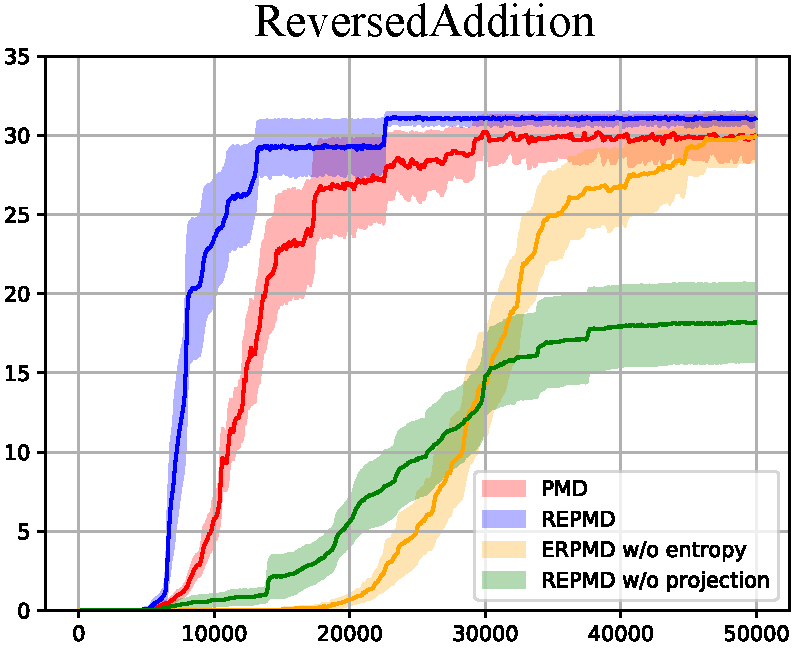
\includegraphics[width=0.35\linewidth]{ablation.pdf}}

\textbf{Importance of entropy regularizer.} The main difference between our objective \cref{eq:pmd} with the original MD is to add another entropy regularizer. We demonstrate the importance of this choice by presenting the results of REPMD with $\tau'=0$.

\textbf{Importance of KL divergence projection.} The main difference between REPMD and the UREX and MENT training methods is to use a projection step to optimize policy rather than performing a single gradient step. To show the importance of the projection step, we reimplement REPMD without projection, which only performs one step of gradient update at each iteration of training. 

\textbf{Importance of direction of KL divergence.} We implemented Policy Mirror Descent (PMD) as another baseline to prove the effectiveness of using the \emph{mean seeking} direction of KL divergence for policy optimization. Like in REPMD, we add a separate tempreture parameter $\tau'\geq 0$ to the original objective function (\ref{eq:max_expected_reward_plus_relative_entropy}) of PMD to encourage further exploration of the policy, which gives $\argmax_{\pi_\theta \in \Pi}{ \ep_{\rho \sim \pi_\theta}{  r(\rho)  - \tau \text{KL}(\pi_\theta \| \refPi) } + \tau'\cH(\pi_\theta) }$.

Results on ReversedAddition are reported in Figure (\ref{fig:ablation}). It clearly shows that optimizing policy by performing the \emph{mean seeking} KL divergence projection is very important as suggested in REPMD. 

\section{Related Work}
\label{related_work}
As mentioned in \cref{sec:pmd}, several existing methods are similar with the policy mirror descent (PMD) framework, by either considering the relative entropy regularizer in policy search/optimization, or using KL divergence as the loss function to optimize the policy. These related works include reward-weighted regression \cite{peters2007reinforcement,wierstra2008episodic}, relative entropy policy search \cite{peters2010relative}, trust region policy optimization \cite{schulman2015trust}, approximate mirror descent policy search \cite{montgomery2016guided}, maximum a posterior policy optimization \cite{abdolmaleki2018maximum}, and soft actor-critic \cite{haarnoja2018soft}. The proposed reversed entropy policy mirror descent (REPMD) method employs a modified version of PMD framework. First, the objective function of PMD is combined with entropy regularizer to enhance further exploration. Second, the projection step applies the \emph{mean seeking} direction of KL divergence instead of the \emph{mean seeking} one used PMD. As shown in both theoretical and practical justification, these two novelties play a very important role in REPMD. 

The Trust PCL method adopts the same objective defined in \cref{eq:repmd}, which includes both entropy and relative entropy regularizer \cite{nachum2017trust}. However, the policy update strategy is different: while REPMD uses KL projection, Trust PCL inherits the same idea from PCL that minimizes path inconsistency error between value and policy for any trajectories \cite{nachum2017bridging}. Although policy optimization by minimizing path inconsistency error can efficiently utilize off-policy data, it is not justified that this method can guarantee policy improvement during learning. On the other hand, the proposed REPMD method can monotonically increase the softmax approximated expected reward, as shown in \cref{sec:repmd}.

\section{Conclusion and Future Work}

In this paper, we have proposed the reversed entropy policy mirror descent (REPMD) method for policy based reinforcement learning, which guarantees monotonic improvement in a well motivated objective. We show that the resulting method achieves better exploration than both a directed exploration method (UREX) and undirected maximum entropy exploration (MENT). It would be interesting to further extend the REPMD method within the actor-critic framework, by developing proper value function learning approach. %In particular, an actor-critic framework would also allow REPMD to perform important sampling on each step without heavy rollouts.


{\small
\bibliographystyle{plain}
\bibliography{nips2018bib}
}

\end{document}
